% !TeX program = pdflatex
\documentclass[tikz,border=8pt]{standalone}
\usepackage{pgfplots}
\pgfplotsset{compat=1.16}
\definecolor{FigureBlue}{HTML}{2563EB}
\definecolor{FigureOrange}{HTML}{EA580C}
\definecolor{FigureGreen}{HTML}{16A34A}
\definecolor{FigureSlate}{HTML}{64748B}
\begin{document}
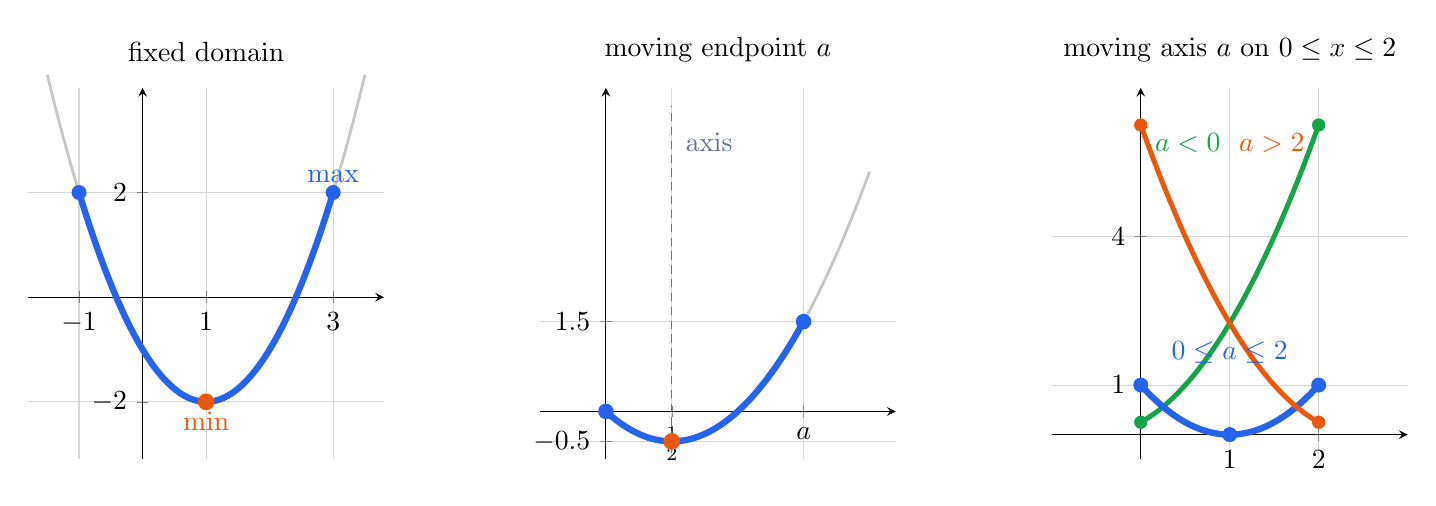
\begin{tikzpicture}
  \begin{axis}[
    width=6.1cm,height=6.3cm,axis lines=middle,xmin=-1.8,xmax=3.8,ymin=-3.1,ymax=4,
    title={fixed domain},xtick={-1,1,3},ytick={-2,2},grid=both,clip=false,
    grid style={draw=gray!18},major grid style={draw=gray!32},
  ]
    \addplot[gray!45,line width=1pt,domain=-1.5:3.5,samples=121] {(x-1)^2-2};
    \addplot[FigureBlue,line width=2.3pt,domain=-1:3,samples=121] {(x-1)^2-2};
    \addplot[only marks,mark=*,mark size=2.5pt,FigureBlue] coordinates {(-1,2) (3,2)};
    \addplot[only marks,mark=*,mark size=2.8pt,FigureOrange] coordinates {(1,-2)};
    \node[anchor=north,text=FigureOrange] at (axis cs:1,-2) {min};
    \node[anchor=south,text=FigureBlue] at (axis cs:3,2) {max};
  \end{axis}
  \begin{axis}[
    at={(6.5cm,0)},anchor=south west,width=6.1cm,height=6.3cm,axis lines=middle,
    xmin=-.5,xmax=2.2,ymin=-.8,ymax=5.4,title={moving endpoint $a$},
    xtick={0,.5,1.5},xticklabels={$0$,$\frac12$,$a$},ytick={-.5,0,1.5},grid=both,clip=false,
    grid style={draw=gray!18},major grid style={draw=gray!32},
  ]
    \addplot[gray!45,line width=1pt,domain=0:2,samples=121] {2*x^2-2*x};
    \addplot[FigureBlue,line width=2.3pt,domain=0:1.5,samples=121] {2*x^2-2*x};
    \addplot[only marks,mark=*,mark size=2.6pt,FigureBlue] coordinates {(0,0) (1.5,1.5)};
    \addplot[only marks,mark=*,mark size=2.8pt,FigureOrange] coordinates {(.5,-.5)};
    \draw[FigureSlate,densely dashed] (axis cs:.5,-.7)--(axis cs:.5,5.1);
    \node[anchor=west,text=FigureSlate] at (axis cs:.53,4.5) {axis};
  \end{axis}
  \begin{axis}[
    at={(13cm,0)},anchor=south west,width=6.1cm,height=6.3cm,axis lines=middle,
    xmin=-1,xmax=3,ymin=-.5,ymax=7,title={moving axis $a$ on $0\le x\le2$},
    xtick={0,1,2},ytick={0,1,4},grid=both,clip=false,
    grid style={draw=gray!18},major grid style={draw=gray!32},
  ]
    \addplot[FigureGreen,line width=1.8pt,domain=0:2,samples=101] {(x+0.5)^2};
    \addplot[FigureBlue,line width=2.3pt,domain=0:2,samples=101] {(x-1)^2};
    \addplot[FigureOrange,line width=1.8pt,domain=0:2,samples=101] {(x-2.5)^2};
    \addplot[only marks,mark=*,mark size=2.2pt,FigureGreen] coordinates {(0,.25) (2,6.25)};
    \addplot[only marks,mark=*,mark size=2.5pt,FigureBlue] coordinates {(0,1) (1,0) (2,1)};
    \addplot[only marks,mark=*,mark size=2.2pt,FigureOrange] coordinates {(0,6.25) (2,.25)};
    \node[anchor=south west,text=FigureGreen] at (axis cs:.05,5.5) {$a<0$};
    \node[anchor=south,text=FigureBlue] at (axis cs:1,1.25) {$0\le a\le2$};
    \node[anchor=south east,text=FigureOrange] at (axis cs:1.95,5.5) {$a>2$};
  \end{axis}
\end{tikzpicture}
\end{document}
